\documentclass{standalone}
\usepackage{pgfplots,relsize}
\usepackage{tikz-3dplot}
\pgfplotsset{compat=1.17}

\begin{document}
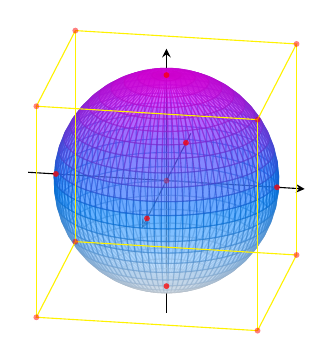
\begin{tikzpicture}
    \begin{axis}[
            view={100}{20},
            % hide axis,
            axis lines = middle,
            ticks = none,
            colormap/cool,
            scale mode = scale uniformly,
            xmin=-10, xmax=10,
            ymin=-10, ymax=10,
            zmin=-10, zmax=10,
        ]

        \addplot3[%
            opacity = 0.5,
            surf,
            z buffer = sort,
            samples = 50,
            variable = \u,
            variable y = \v,
            domain = 0:180,
            y domain = 0:360,
        ]
        ({8*cos(u)*sin(v)}, {8*sin(u)*sin(v)}, {8*cos(v)});

        \draw[yellow] (-8,-8,-8) -- (-8,8,-8) -- (8,8,-8) -- (8,-8,-8) -- cycle;
        \draw[yellow] (-8,-8,8) -- (-8,8,8) -- (8,8,8) -- (8,-8,8) -- cycle;

        %draw the edges of the cube
        \draw[yellow] (-8,-8,-8) -- (-8,-8,8);
        \draw[yellow] (-8,8,-8) -- (-8,8,8);
        \draw[yellow] (8,-8,-8) -- (8,-8,8);
        \draw[yellow] (8,8,-8) -- (8,8,8);


        \node[opacity= .5, red, circle, fill, inner sep=0.75pt] at (-8, -8, -8) {};
        \node[opacity= .5, red, circle, fill, inner sep=0.75pt] at (-8, -8,  8) {};
        \node[opacity= .5, red, circle, fill, inner sep=0.75pt] at (-8,  8, -8) {};
        \node[opacity= .5, red, circle, fill, inner sep=0.75pt] at (-8,  8,  8) {};
        \node[opacity= .5, red, circle, fill, inner sep=0.75pt] at ( 8, -8, -8) {};
        \node[opacity= .5, red, circle, fill, inner sep=0.75pt] at ( 8, -8,  8) {};
        \node[opacity= .5, red, circle, fill, inner sep=0.75pt] at ( 8,  8, -8) {};
        \node[opacity= .5, red, circle, fill, inner sep=0.75pt] at ( 8,  8,  8) {};


        \node[opacity=.75, red, circle, fill, inner sep=0.75pt] at ( 8,  0,  0) {};
        \node[opacity=.75, red, circle, fill, inner sep=0.75pt] at ( 0,  8,  0) {};
        \node[opacity=.75, red, circle, fill, inner sep=0.75pt] at ( 0,  0,  8) {};
        \node[opacity=.75, red, circle, fill, inner sep=0.75pt] at (-8,  0,  0) {};
        \node[opacity=.75, red, circle, fill, inner sep=0.75pt] at ( 0, -8,  0) {};
        \node[opacity=.75, red, circle, fill, inner sep=0.75pt] at ( 0,  0, -8) {};

        \node[opacity= .3, red, circle, fill, inner sep=0.75pt] at ( 0,  0,  0) {};
    \end{axis}
\end{tikzpicture}
\end{document}